\chapter{滾動標量場引發的暴脹}

\lectureoverview{上一講留下的一個問題，為本講提供了主軸方程：
\(\ddot\phi+3H\dot\phi=-V'(\phi)\)：什麼在運動？什麼施加作用力？為什麼膨脹會像摩擦？我們先在固定盒子中推導這個方程，再推導膨脹盒子中的情形。將它與弗里德曼方程結合，便得到慢滾機制：高而平緩的標量勢驅動近乎指數的膨脹。暴脹會稀釋磁單極子並抹平幾何；暴脹結束時，宇宙再加熱，傳統的熱大爆炸階段由此開始。接著便無可避免地要問：如果暴脹如此有效地抹平宇宙，結構又從何而來？一維焦散計算顯示，微小的速度變化如何形成片層、絲狀結構和節點；至於這些變化的量子起源，則留待下一講討論。}

\section{什麼作用於什麼？}

開場的問題回顧了方程
\begin{equation}
\ddot\phi+3H\dot\phi
=F(\phi)
=-\frac{dV}{d\phi}
\label{eq:c09-opening}
\end{equation}
並追問什麼樣的力\(F\)能作用在場上。這不是枝節問題。要回答它，我們必須重建場的力學；而這也正是暴脹這個主題的起點。

標量場在每個空間和時間位置都指定一個數值\(\phi(\mathbf x,t)\)。電場和磁場攜帶能量，標量場也能攜帶能量。這裡需要的場是假設性的：目前尚未透過實驗辨認出任何特定的暴脹子，因此其能量如何隨場值變化仍然未知。我們以一個未具體指定的勢能密度表示它：
\begin{equation}
V=V(\phi).
\label{eq:c09-potential}
\end{equation}
\(\phi\)的不同取值，對應於每單位物理體積中儲存的不同能量。

沒有理由認為\(\phi=0\)的能量必為零。場空間的原點只是一種約定，對尚未發現的場尤其如此；改變標記場值的座標，不必把\(V\)的極小值放在原點。\(V(\phi)\)的圖形描述的是相對的斜率和高度，並沒有指定場的某個特別起點。

勢能是場瞬間靜止時所具有的能量部分。如果場隨時間變化，它也有動能。\(\dot\phi\)不是物體在一般空間中的速度，而是場值的變化率，也就是場空間中的速度。彈性弦是個有用的類比：弦的位移是定義在一維世界上的場，而振動的弦元所帶的動能，正比於其時間導數的平方。

平方項前的係數可以吸收到場的定義中。若一開始寫成
\begin{equation}
\frac12 n^2\dot\phi^{\,2},
\end{equation}
再作變數變換
\begin{equation}
\chi=n\phi
\end{equation}
這一項就會變成\(\dot\chi^{\,2}/2\)。因此，我們可以選用正則歸一化的場，並在均勻近似下寫成
\begin{equation}
\rho_\phi=\frac12\dot\phi^{\,2}+V(\phi).
\label{eq:c09-rho-homogeneous}
\end{equation}
這只是對場空間座標作歸一化，並不是說某個字面上的粒子質量被設為一。

\section{固定盒子中的力學}

考慮一個小盒子，其中的場在空間中幾乎均勻。它的能量密度在數學形式上與單位質量粒子的能量相同：動能加上勢能。相應的拉格朗日密度中，勢能項的符號相反：
\begin{equation}
\mathcal L_\phi
=\frac12\dot\phi^{\,2}-V(\phi).
\label{eq:c09-lagrangian-density}
\end{equation}
這只是數學上的類比。廣義座標是場值，而不是粒子的空間位置。

尤拉--拉格朗日方程為
\begin{equation}
\frac{d}{dt}
\left(
\frac{\partial\mathcal L_\phi}{\partial\dot\phi}
\right)
=
\frac{\partial\mathcal L_\phi}{\partial\phi}.
\label{eq:c09-el-fixed}
\end{equation}
此處的速度變數是\(\dot\phi\)，因此
\begin{equation}
\frac{\partial\mathcal L_\phi}{\partial\dot\phi}=\dot\phi,
\qquad
\frac{\partial\mathcal L_\phi}{\partial\phi}=-V'(\phi),
\end{equation}
可得
\begin{equation}
\ddot\phi=-V'(\phi)\equiv F(\phi).
\label{eq:c09-fixed-eom}
\end{equation}
二階導數是場座標的加速度，而勢能的負斜率就是作用在它上面的力。

\begin{figure}[htbp]
\centering
\includegraphics[width=0.88\textwidth]{lecture_09_figure_03.png}
\caption{黑板上可辨識的部分，將\(V(\phi)\)帶入固定盒子的方程\(\ddot\phi=-\partial V/\partial\phi\)。上方的尤拉--拉格朗日表示式有一部分被裁切或遮住，因此方程~\eqref{eq:c09-el-fixed}是根據推導重建的，並非照錄一個完整呈現的畫面。}
\label{fig:c09-fixed-board}
\lectureframe{00:10:53.836}
\end{figure}

\begin{classroomqa}
\audiencequestion{力是什麼？它作用在什麼上？}
\lecturerresponse{演化的對象是標量值\(\phi\)。\(-V'(\phi)\)是在場空間中的力：它使場值朝勢能較低的方向加速，正如\(-dV/dx\)使粒子座標加速一樣。它不是一種新的向量力，將物質物體推動穿越一般空間。\lecturetimestamp{00:00:27--00:00:49; 00:10:41--00:11:29}}
\end{classroomqa}

完整的場可以隨空間位置而變化。在空間平坦的膨脹幾何中，正則標量場的局部能量密度包含
\begin{equation}
\rho_\phi
=
\frac12\dot\phi^{\,2}
+\frac{1}{2a^2}\lvert\nabla\phi\rvert^2
+V(\phi).
\label{eq:c09-rho-full}
\end{equation}
我們忽略梯度項，因為膨脹會把場的變化拉伸到長波長，使小盒子內的場近乎均勻。這是根據宇宙學情境所作的近似，並非否認標量波或空間漣漪的存在。

\section{膨脹中的盒子}

第一次推導回答了開場的問題，但還不是宇宙學中的推導。方程~\eqref{eq:c09-rho-homogeneous}和\eqref{eq:c09-lagrangian-density}描述的是密度。單位共動盒子的物理體積正比於\(a^3(t)\)，因此它的拉格朗日量為
\begin{equation}
L_\phi
=a^3(t)
\left[
\frac12\dot\phi^{\,2}-V(\phi)
\right].
\label{eq:c09-comoving-lagrangian}
\end{equation}
因子\(a^3\)在靜止的盒子中無關緊要；在宇宙學中，它會隨時間變化，而正是這種時間依賴補上了缺少的那一項。

\begin{figure}[htbp]
\centering
\includegraphics[width=0.88\textwidth]{lecture_09_figure_04.png}
\caption{左側可見手繪的勢能曲線，右側則有能量與拉格朗日量表示式的片段。曲線形狀和符號變化都可以確認；方程~\eqref{eq:c09-comoving-lagrangian}的完整代數式則來自口述推導，因為講者遮住了部分黑板。}
\label{fig:c09-potential-board}
\lectureframe{00:13:26.528}
\end{figure}

將尤拉--拉格朗日方程套用於\(L_\phi\)，可得
\begin{align}
\frac{d}{dt}\left(a^3\dot\phi\right)
&=-a^3V'(\phi), \label{eq:c09-a3-form}\\
a^3\ddot\phi+3a^2\dot a\,\dot\phi
&=-a^3V'(\phi),\\
\ddot\phi+3\frac{\dot a}{a}\dot\phi
&=-V'(\phi).
\end{align}
代入\(H=\dot a/a\)後，結果為
\begin{equation}
\boxed{\ddot\phi+3H\dot\phi=-V'(\phi)}.
\label{eq:c09-hubble-friction}
\end{equation}
開場時回憶的方程，現在已經推導出來，而不只是被重新提起。

\begin{figure}[htbp]
\centering
\includegraphics[width=0.96\textwidth]{lecture_09_figure_05.png}
\caption{左側是固定盒子的動力學，右側則是膨脹盒子帶來的修正。黑板上可見的內容呈現了從\(d(a^3\dot\phi)/dt\)到\(3\dot a/a\)及\(3H\)形式的推導次序；右側被裁切的部分則由方程~\eqref{eq:c09-a3-form}補足。}
\label{fig:c09-expanding-board}
\lectureframe{00:18:35.380}
\end{figure}

\begin{classroomqa}
\audiencequestion{力\(F\)可以用更具體的方式來想像嗎？}
\lecturerresponse{把\(V(\phi)\)想成一片地形，水平座標代表場值。斜率決定作用力：\(F=-V'(\phi)\)。向下的斜坡越陡，場空間中的驅動力越大；斜坡越平緩，驅動力就越小。這個圖像只是幫助理解一維場座標，並不表示物理空間中真的有一座山。\lecturetimestamp{00:18:26--00:19:18}}
\end{classroomqa}

\section{哈伯摩擦與終端運動}

把方程~\eqref{eq:c09-hubble-friction}中的中間項移到右側：
\begin{equation}
\ddot\phi=-V'(\phi)-3H\dot\phi.
\end{equation}
在膨脹宇宙中\(H>0\)，第二項的作用方向永遠與場的速度相反，因此它的效果就像黏滯阻力。石頭放進濃稠的蜂蜜中後會先加速，但阻力會隨速度增加，直到石頭達到終端速度。\emph{\(H\)}這個蜂蜜記憶法抓住了類比的要點，而方程則給出它的實際內容。如果\(H\)隨宇宙時間變化，有效黏滯阻力也會跟著變化，就像一般的黏滯性會隨溫度改變一樣。

當摩擦效應遠大於慣性效應時，\(\lvert\ddot\phi\rvert\ll3H\lvert\dot\phi\rvert\)，場便會迅速趨近於
\begin{equation}
3H\dot\phi\simeq -V'(\phi),
\qquad
\dot\phi\simeq-\frac{V'(\phi)}{3H}.
\label{eq:c09-terminal}
\end{equation}
平緩的勢能斜率帶來較小的力，而較大的\(H\)則帶來較強的阻力。這兩種效應都會使\(\dot\phi\)變小，通常也會使動能密度\(\dot\phi^2/2\)遠小於\(V\)。

\begin{classroomqa}
\audiencequestion{這個推導是否依賴最小作用量原理？}
\lecturerresponse{是。方程~\eqref{eq:c09-hubble-friction}是將由方程~\eqref{eq:c09-comoving-lagrangian}建立的作用量取極值得出的。也可以把場方程直接當作動力學定律的起點；不過，變分推導恰好說明了為什麼膨脹體積會貢獻出\(3H\dot\phi\)。\lecturetimestamp{00:25:40--00:26:15}}
\end{classroomqa}

\begin{classroomqa}
\audiencequestion{如果新增的項像摩擦，那麼損失的能量去了哪裡？}
\lecturerresponse{石頭在蜂蜜中運動時，會把機械能轉化為熱。宇宙學中的情況更微妙。共動盒子的拉格朗日量透過\(a(t)\)顯式地依賴時間，因此盒子的普通機械能不會因時間平移對稱性而守恆。局部協變的應力能量守恆仍然成立：
\[
\dot\rho_\phi+3H(\rho_\phi+p_\phi)=0,
\qquad
p_\phi=\frac12\dot\phi^{\,2}-V(\phi).
\]
對均勻標量場而言，這會化為\(\dot\rho_\phi=-3H\dot\phi^{\,2}\)：場對膨脹中的幾何做功。失效的是把演化中的宇宙視為具有樸素的全域守恆能量，而非應力能量的局部守恆。\lecturetimestamp{00:26:16--00:27:57}}
\end{classroomqa}

\section{場驅動膨脹}

到目前為止，我們看到的是膨脹如何作用在標量場上。這只是回饋機制的一半。標量場的能量密度也會透過平直空間中的弗里德曼方程決定膨脹：
\begin{equation}
H^2=\left(\frac{\dot a}{a}\right)^2
=\frac{8\pi G}{3}\rho.
\label{eq:c09-friedmann}
\end{equation}
對於近乎均勻的標量場，
\begin{equation}
H^2
=\frac{8\pi G}{3}
\left[
\frac12\dot\phi^{\,2}+V(\phi)
\right].
\label{eq:c09-friedmann-scalar}
\end{equation}
膨脹會使場受到阻尼，而受到阻尼的場又能反過來維持驅動膨脹的能量密度。

\begin{classroomqa}
\audiencequestion{這個假設性的標量場就是所謂的暴脹子嗎？}
\lecturerresponse{是。這個名稱指的是賦予它的角色：勢能近乎不變、並驅動暴脹的標量場。為場命名並不代表已確定其粒子物理本質。暴脹子的具體種類、它的耦合方式，甚至是否由單一基本標量場扮演這個角色，都取決於模型。\lecturetimestamp{00:30:26--00:31:28}}
\end{classroomqa}

\begin{classroomqa}
\audiencequestion{有暴脹子的實驗證據嗎？}
\lecturerresponse{目前尚未在實驗室直接探測到任何特定的暴脹子場。現有證據是間接的：暴脹動力學為觀測到的平坦性與原初擾動提供了一套成功的架構，但許多不同的勢能都能符合這些概括性的觀測事實。這種間接支持，應與對微觀實現方式的了解區分開來。\lecturetimestamp{00:31:29--00:33:02}}
\end{classroomqa}

\begin{classroomqa}
\audiencequestion{所有場都攜帶能量嗎？標量場的激發會是玻色子嗎？}
\lecturerresponse{物理場會貢獻能量與動量。將標量場量子化後，會得到自旋為零的玻色子量子。描述暴脹的經典均勻背景，不宜想成一個普通粒子；不過暴脹結束後，它的振盪可以用暴脹子量子來描述。\lecturetimestamp{00:33:03--00:35:20}}
\end{classroomqa}

\begin{classroomqa}
\audiencequestion{希格斯場可能是暴脹子嗎？}
\lecturerresponse{理論上需要的是標量場，因此這種類比很自然；但觀測到的希格斯場，連同其標準模型中的一般勢能與耦合，並不會自動成為這個簡單平臺所描述的場。希格斯暴脹模型會加入非最小引力結構。目前的論證沒有任何內容能將暴脹子認定為希格斯場。\lecturetimestamp{00:35:21--00:37:11}}
\end{classroomqa}

現在設想\(V(\phi)\)在一段很長的區間內既很高又只有緩慢的斜率。方程~\eqref{eq:c09-terminal}使場緩慢移動，因此
\begin{equation}
\frac12\dot\phi^{\,2}\ll V(\phi).
\end{equation}
弗里德曼方程便簡化為
\begin{equation}
H^2\simeq\frac{8\pi G}{3}V(\phi),
\qquad
H\simeq
\sqrt{\frac{8\pi G}{3}V(\phi)}.
\label{eq:c09-potential-dominated}
\end{equation}
導數\(V'(\phi)\)控制場的緩慢運動；勢能的高度\(V(\phi)\)則控制空間快速膨脹。

\begin{figure}[htbp]
\centering
\includegraphics[width=0.92\textwidth]{lecture_09_figure_06.png}
\caption{弗里德曼方程、標量場的能量密度，以及以方框標示的勢能主導表示式。\(V(\phi)\)中的平方根項清晰可見；方程~\eqref{eq:c09-potential-dominated}中開頭的\(H\simeq\)則是根據口述論證補全的標準形式。}
\label{fig:c09-friedmann-board}
\lectureframe{00:41:04.178}
\end{figure}

如果場經過平臺時\(V\)只略有變化，\(H\)就會近乎恆定。對\(\dot a/a\simeq H\)積分可得
\begin{equation}
a(t)\simeq a_i e^{H(t-t_i)}.
\label{eq:c09-exponential}
\end{equation}
這就是暴脹。早期宇宙的倍增時間約為\(10^{-32}\,\mathrm{s}\)，足以呈現暴脹的劇烈程度；這個數字僅供說明，實際數值取決於暴脹能量尺度。

\begin{classroomqa}
\audiencequestion{場移動得很慢，怎麼能使宇宙快速膨脹？}
\lecturerresponse{移動緩慢的是\(\phi\)，不是\(a\)。哈伯摩擦阻止場沿著勢能快速下滑，因此\(V(\phi)\)幾乎保持不變。很大且近乎不變的\(V\)會帶來很大且近乎不變的\(H\)，於是尺度因子便呈指數增長。微弱的斜率控制場的運動；高聳的平臺控制宇宙的膨脹。\lecturetimestamp{00:40:06--00:41:39}}
\end{classroomqa}

\section{為什麼要引入暴脹？}

暴脹由阿蘭・古斯於1980年前後提出，用來解決具體的宇宙學問題。後續研究，尤其是安德烈・林德等人的工作，發展出能讓暴脹階段平順結束的模型。這個整體架構符合許多重要觀測，但目前尚未確立唯一的勢能；不能因為這套機制成功，就宣稱每個細節都已獲得實驗證實。

\subsection{磁單極子問題}

大統一理論通常容許磁單極子存在。粗略估計顯示，它們的質量大得驚人，可能比質子質量高出許多個數量級；確切質量取決於理論，不一定恰好等於普朗克質量。足夠高溫的早期宇宙會透過熱產生磁單極子--反磁單極子對。宇宙冷卻後，磁荷會使這些遺留下來的粒子繼續存在。

觀測中並沒有發現可觀的磁單極子遺跡密度。特別是，自由運動的磁荷會有效耗散星系磁場，就像可移動的電荷會屏蔽或中和電場。因此，星系磁場至今仍然存在，對宇宙中的磁單極子數量形成了嚴格限制。暴脹透過將體積放大極大的倍數來解決這個問題：暴脹前存在的磁單極子會被稀釋，直到我們的可觀測區域內幾乎不剩任何磁單極子。

\subsection{均勻性與平坦性}

宇宙微波背景極為均勻。若沒有暴脹，依照最簡單的熱大爆炸模型向前推演，最後散射面上相距遙遠的區域彼此之間幾乎沒有因果接觸，難以解釋為什麼它們的溫度如此接近。暴脹從一個小得多、彼此具有因果聯繫的區域開始，並將它拉伸至涵蓋可觀測宇宙。它也會使空間曲率趨近於零，類似於一個極度膨脹的球面上，小區域看起來近乎平坦。

膨脹程度以\(e\)倍數的折數衡量：
\begin{equation}
N\equiv \ln\frac{a_{\rm end}}{a_{\rm start}}
=\int_{t_{\rm start}}^{t_{\rm end}}H\,dt.
\label{eq:c09-efolds}
\end{equation}
我們將以\(N\gtrsim60\)作為實用的數量級下限。所需的確切折數取決於暴脹能量尺度與再加熱歷史；不同模型的估計值廣泛分布於\(40\)--\(80\)附近。初始狀態若更不平滑，或遺跡密度若更高，都可能需要更多暴脹。

\begin{classroomqa}
\audiencequestion{如果宇宙的初始狀態完全混沌，六十個\(e\)折仍然足夠嗎？}
\lecturerresponse{不一定。在特定假設下，六十是解決標準視界與平坦性問題時常用的下限估計。初始狀態若更不平滑，可能需要更長的平緩平臺。這並不表示有一個放諸四海皆準的整數，可以消除所有可能的初始條件。\lecturetimestamp{00:55:23--00:56:48}}
\end{classroomqa}

\begin{classroomqa}
\audiencequestion{暴脹持續時間有觀測上的上限嗎？}
\lecturerresponse{單憑目前的討論，無法推得類似的直接上限。暴脹一旦持續得夠久，額外的\(e\)折便會使曲率和原先存在的遺跡更難被觀測到。要產生極長的暴脹階段，可能需要相應地拓寬勢能並精細安排其形狀；但那是模型建構上的代價，而非測量所得的上限。\lecturetimestamp{00:56:49--00:58:45}}
\end{classroomqa}

如果暴脹持續的時間只比所需下限略長，殘餘曲率可能仍在未來的觀測能力範圍內。因此，隨著曲率測量持續改進，我們可以探查暴脹拉伸是否接近最低需求，或是長得多；不過，即使沒有測得曲率，也無法確定\(N\)究竟有多大。

\begin{classroomqa}
\audiencequestion{空間暴脹時，溫度會如何變化？}
\lecturerresponse{一般粒子和輻射會被稀釋並發生紅移，因此從熱力學的角度來看，宇宙會變得極度寒冷而空曠。但宇宙並非毫無能量：近乎不變的標量勢能仍然存在，並驅動膨脹。暴脹結束後，必須重新形成熱宇宙。\lecturetimestamp{00:59:49--01:01:10}}
\end{classroomqa}

\section{離開平臺}

如果平臺永遠平坦，宇宙便會永遠膨脹，且不會有一般物質。因此，勢能的性質必須有所改變。一個示意性的圖像是：先有一段長而平緩的區域，接著是較陡的下降，最後到達一個極小值：
\begin{figure}[htbp]
\centering
\begin{coursefitfigure}
\begin{tikzpicture}[x=1.05cm,y=0.95cm,>=Latex]
  \draw[->] (-0.2,0) -- (10.2,0) node[right] {\(\phi\)};
  \draw[->] (0,-0.2) -- (0,4.5) node[above] {\(V(\phi)\)};
  \draw[very thick,blue!55!black]
    plot[smooth] coordinates {
      (0.3,3.8) (1.4,3.72) (2.6,3.63) (3.8,3.52)
      (4.8,3.25) (5.5,2.45) (6.1,1.18) (6.8,0.45)
      (7.5,0.18) (8.2,0.32) (9.1,0.27) (9.8,0.27)
    };
  \draw[->,thick,red!65!black] (2.0,4.15) -- (3.1,4.02);
  \node[above] at (2.55,4.12) {slow roll};
  \draw[dashed] (6.2,0) -- (6.2,2.3);
  \node[align=center] at (6.1,3.05) {end of\\inflation};
  \draw[->,thick,red!65!black] (6.2,2.15) -- (6.75,0.82);
  \node[align=center,below] at (7.5,-0.15) {damped oscillation\\and reheating};
  \node[right] at (8.7,0.55) {small residual \(V_{\min}\)};
\end{tikzpicture}
\end{coursefitfigure}
\caption{暴脹勢能的示意圖：高而平緩的平臺、陡峭的出口，以及受到阻尼而逐漸趨近極小值的振盪。勢能的詳細形狀尚不清楚；此曲線只呈現論證所需的定性階段。}
\label{fig:c09-inflation-potential}
\end{figure}

當\(\phi\)接近下降區域時，\(V\)隨之減小，因此\(H\)也會減小，而\(\lvert V'(\phi)\rvert\)則會增大。下坡的力愈來愈強，蜂蜜卻同時變得愈來愈稀。慢滾近似不再成立，場開始加速，暴脹也隨之結束。自然界為什麼會提供這樣的勢能，以及場最初為什麼會位於平臺上，都無法只靠畫出這條曲線來解釋。這些仍是微觀理論及其初始條件所留下的問題。

\begin{classroomqa}
\audiencequestion{暴脹是在光子退耦附近開始的嗎？}
\lecturerresponse{不是。暴脹發生在極早期宇宙。退耦則發生在之後的熱大爆炸階段，當時距離該階段開始已有數十萬年；在此之前還經歷了再加熱、核合成和漫長的膨脹。這兩件事之間相隔了極長的宇宙歷史。\lecturetimestamp{01:03:33--01:04:39}}
\end{classroomqa}

\subsection{再加熱}

場往下移動時，其勢能會轉化為相干動能，場也會在極小值附近振盪。場與其他場的耦合可以把能量轉移給粒子；粒子經過散射後，會逐漸趨近熱分佈。這個過程稱為再加熱。它產生光子、電子、正電子、夸克及其他粒子，進而形成傳統大爆炸圖像中的初始熱電漿。因此，熱大爆炸本身不是暴脹狀態，而是暴脹結束後的結果。

\begin{classroomqa}
\audiencequestion{再加熱是否類似希格斯場產生光子和物質？}
\lecturerresponse{有用的類比是：激發態的場會衰變為與它耦合之其他場的量子。暴脹子的振盪可以產生暴脹子量子，而這些激發態則可以衰變成較輕的粒子。哪些粒子會直接出現、哪些會在後續反應中產生，以及希格斯場是否參與其中，都取決於具體模型。\lecturetimestamp{01:06:02--01:08:18}}
\end{classroomqa}

\begin{classroomqa}
\audiencequestion{暴脹是否表示空間從一個點開始，然後膨脹到某種外部空間中？}
\lecturerresponse{不需要假設有外部空間。可以把微小的封閉三維空間當作輔助想像，但宇宙不是向周圍房間膨脹的普通球體。暴脹放大的是空間內的物理距離。暴脹本身也無法確立宇宙有一個絕對起點；它描述的是暴脹條件成立後，一個區域如何演化。\lecturetimestamp{01:08:19--01:11:49}}
\end{classroomqa}

\section{位於極小值時：真空能與未解問題}

如果極小值仍保有微小的正值\(V_{\min}\)，它的效果就如同宇宙學常數。同一個廣義的標量勢能圖像，因而可以把原初暴脹時期和現在的加速膨脹時期放在同一張圖上。這是課堂上簡潔的可能圖像，並非證據表明今天的暗能量就是原初暴脹子留下的能量。

\begin{classroomqa}
\audiencequestion{如果沒有找到磁單極子，是否就必須提高\(e\)折的最低數目？}
\lecturerresponse{這裡討論的未來觀測目標是殘餘空間曲率，而不是近期探測磁單極子。現有的磁場論證已使大量磁單極子存在的可能性很低。若曲率的零結果限制更加嚴格，暴脹所需折數的下限就會提高，因為膨脹得愈多，空間就愈平坦。這些都是暴脹帶來的相關結果，但並非同一種測量。\lecturetimestamp{01:12:37--01:14:06}}
\end{classroomqa}

\begin{classroomqa}
\audiencequestion{底部這麼少的能量就是今天的真空能嗎？}
\lecturerresponse{在這個示意圖像中，是的：\(V_{\min}\)是目前真空態的能量，並發揮宇宙學常數的作用。這個能量階層極為懸殊，比自然的普朗克尺度估計值低約\(120\)個數量級，也遠低於典型的暴脹能量密度。這個引人入勝的統一圖像並未解釋這個數值。\lecturetimestamp{01:14:07--01:14:56}}
\end{classroomqa}

\begin{classroomqa}
\audiencequestion{如果暴脹一開始就讓宇宙變得空無一物，那麼究竟什麼被抹平了？磁單極子又是在什麼時候被移除的？}
\lecturerresponse{暴脹會使空間幾何變得平滑、平坦，並稀釋當時已存在的粒子或磁單極子。如果後續的能量釋放把宇宙加熱到高於磁單極子生成門檻的溫度，問題就會再次出現。因此，必須一併安排時間順序和能量尺度，不能把幾何平滑與再加熱視為彼此獨立的過程。\lecturetimestamp{01:14:58--01:16:38}}
\end{classroomqa}

再加熱必須拿捏得恰到好處：溫度必須高到足以產生後續宇宙所需的粒子，卻又不能高到使暴脹剛稀釋掉的磁單極子再度生成。這也是為什麼不能脫離粒子物理學，單獨指定暴脹如何結束。

\begin{classroomqa}
\audiencequestion{磁單極子是粒子嗎？它們一定是在暴脹前就存在嗎？}
\lecturerresponse{磁單極子是極重、類似粒子的激發態，帶有磁荷。它們可能曾經存在，後來被稀釋；也可能是暴脹前的狀態從未熱到足以產生它們。必須避免的是暴脹後的熱浴溫度高到足以再次大量生成磁單極子。\lecturetimestamp{01:16:41--01:17:09}}
\end{classroomqa}

場可能越過極小值，來回振盪；但哈伯摩擦和粒子生成會使這些振盪逐漸阻尼。在簡單的圖像中，場會停留在底部附近，而不會無止盡地爬上另一側。

\begin{classroomqa}
\audiencequestion{勢能為什麼不再平坦，而突然下降？}
\lecturerresponse{目前還不知道。這條曲線只是用來描述觀測所要求的動力學，並沒有解釋自身的形狀。有人提出人擇選擇，作為探討為何宜居區域具有適當真空能和宇宙歷史的一種可能方式；但目前不知道這是否是正確的解釋，而且在此並沒有推導出任何暴脹子的勢能。\lecturetimestamp{01:17:33--01:19:22}}
\end{classroomqa}

\begin{classroomqa}
\audiencequestion{說原因未知，是否表示這個變化沒有原因？}
\lecturerresponse{不能由此得出這樣的結論。這只表示目前不知道負責此事的微觀理論。不知道原因，並不代表變化沒有原因。\lecturetimestamp{01:19:23--01:19:59}}
\end{classroomqa}

\begin{classroomqa}
\audiencequestion{勢能圖的橫軸是時間嗎？\(\phi=0\)在哪裡？}
\lecturerresponse{橫座標是\(\phi\)，其零點可以設在任何方便的位置，例如今天的極小值處。時間則標記沿曲線的軌跡\(\phi(t)\)。在\(H\)幾乎不變的慢滾期間，\(N\simeq H\Delta t\)，因此六十個\(e\)折大約相當於六十個哈伯時間，而非六十個場值單位。下降過程可能比一個早期哈伯時間還長，但以一般尺度來看仍然極為迅速。\lecturetimestamp{01:20:00--01:21:45}}
\end{classroomqa}

\begin{classroomqa}
\audiencequestion{場有可能再次爬上勢能的另一側嗎？}
\lecturerresponse{它可能會過衝並振盪幾次，但\(3H\dot\phi\)項會消除它的運動。停在黏滯海底的石頭不會自行升到海面；同樣地，除非有額外擾動提供能量，阻尼中的場在經典情況下不會回到平臺。\lecturetimestamp{01:21:46--01:22:58}}
\end{classroomqa}

\begin{classroomqa}
\audiencequestion{再加熱把宇宙加熱到多高的溫度？}
\lecturerresponse{具體溫度尚不清楚。溫度必須高到足以產生夸克和大量粒子--反粒子對，因此\(10^{11}\)--\(10^{12}\,\mathrm{K}\)只是課堂估算中粗略的低端參考值，並非測量結果。溫度可能高得多，但仍低於會使危險磁單極子重新大量生成的門檻。\lecturetimestamp{01:22:58--01:25:07}}
\end{classroomqa}

\begin{classroomqa}
\audiencequestion{暴脹場是否有相應的玻色子？它們會衰變成什麼？}
\lecturerresponse{將標量場量子化後，會得到暴脹子玻色子。在場下降和振盪的階段，暴脹子的耦合可以產生光子、電子、夸克、其他普通粒子，也可能產生暗物質。具體有哪些粒子以及各自的分支比，取決於尚不清楚的微觀模型；暴脹子的衰變則是場能量轉化為熱浴的機制。\lecturetimestamp{01:25:08--01:25:49}}
\end{classroomqa}

\section{一個隱藏過去的宇宙}

在現今的宇宙中，場被描繪成停留在極小值附近。若其微小的正能量持續存在，宇宙晚期將趨向類德西特膨脹。相較於早期宇宙的暴脹，這種膨脹十分緩慢；但經過極漫長的時間，遙遠且不受引力束縛的星系仍會被帶到因果可及範圍之外。微波背景會冷卻到實際上無法探測的程度，而未來身處局部束縛殘骸中的觀測者，可能會看到一個看似空無一物的宇宙，幾乎沒有更廣大星系族群存在的直接證據。

\begin{classroomqa}
\audiencequestion{宇宙是否起源於某個更大空間中的點源？這樣的點源是否可能不只一個？}
\lecturerresponse{稱它為點源，容易使我們想像有一個嵌入空間，點源就位於其中；這種想像並不正確。微小的封閉三維空間只是對初始幾何的一種啟發式描述，並非外部房間裡的一顆球。更廣泛的理論容許存在多個彼此因果隔離的暴脹區域，但這個模型並未回答是否真有這些區域。\lecturetimestamp{01:30:10--01:30:57}}
\end{classroomqa}

\begin{classroomqa}
\audiencequestion{遙遠未來的這種孤立，是否類似於我們目前無法觀測視界之外的區域？}
\lecturerresponse{是的。兩種情況下，因果邊界都限制了可接收的訊號。對局部觀測者而言，遙遠未來的情況更為極端，因為幾乎所有未與他們形成引力束縛的星系都已越過這道邊界。\lecturetimestamp{01:31:00--01:31:18}}
\end{classroomqa}

\begin{classroomqa}
\audiencequestion{來自遙遠文明的古老無線電訊號，還能被探測到嗎？}
\lecturerresponse{已經在傳播途中的訊號會繼續傳播，但宇宙膨脹會拉長其波長，並降低其能量和抵達頻率。越過事件視界之後才發出的訊號，永遠不會抵達我們。即使是最早發出的廣播，最終也會因紅移而變得無法實際接收。\lecturetimestamp{01:31:18--01:31:42}}
\end{classroomqa}

\begin{classroomqa}
\audiencequestion{一個暴脹子量子有多重？}
\lecturerresponse{對正規化的場而言，小振盪的質量由勢能在極小值附近的曲率決定，
\[
m_\phi^2=V''(\phi_{\min}).
\]
該曲率尚不清楚。目前實驗所支持的概括性說法只有：現有的加速器實驗尚未發現足夠輕、且以通常方式與其他粒子耦合的暴脹子。\lecturetimestamp{01:31:58--01:32:25}}
\end{classroomqa}

\begin{classroomqa}
\audiencequestion{\(\phi\)也會隨位置改變嗎？它最初的漣漪是量子漲落嗎？}
\lecturerresponse{一般而言，\(\phi=\phi(\mathbf x,t)\)。經典的空間漣漪可能被拉伸到波長極長，使場在局部區域內看起來均勻；這就是先前可以忽略\(\nabla\phi\)的理由。量子漲落是另一種效應，並非第一次平滑化論證中所用的經典漣漪。這裡刻意暫不討論量子漲落的作用，因為它們將提供結構形成的種子。\lecturetimestamp{01:32:32--01:33:51}}
\end{classroomqa}

\begin{classroomqa}
\audiencequestion{我們今天應該能看到星系明顯地越過視界嗎？}
\lecturerresponse{不會像看著附近物體穿過一道發光表面那樣。觀測最遙遠的距離，也意味著回望最遙遠的過去，直到星系形成之前不透明的最後散射面。遙遠星系後來發出的訊號會逐漸變得更紅、更暗；視界是因果邊界，不是物質外殼。\lecturetimestamp{01:33:52--01:34:50}}
\end{classroomqa}

\begin{classroomqa}
\audiencequestion{足夠有耐心的未來觀測者，能否找回宇宙膨脹的證據？}
\lecturerresponse{一旦只剩下一個引力束縛的星系殘骸，直接天文觀測將極為困難。原則上，探測器和長基線訊號交換可以在數十億年間測量幾何、退行和曲率。不過，探測器必須在越過事件視界之前折返，否則便無法傳回任何報告。\lecturetimestamp{01:34:51--01:37:11}}
\end{classroomqa}

\begin{classroomqa}
\audiencequestion{暗能量會摧毀資訊嗎？}
\lecturerresponse{這項經典論證並未導出資訊遭到摧毀的結論。暗能量可以將資訊來源帶到視界之外，使特定觀測者在實際操作上無法取得資訊。基本層次的資訊遺失則是另一個量子重力問題。\lecturetimestamp{01:37:12--01:37:20}}
\end{classroomqa}

\begin{classroomqa}
\audiencequestion{仙女座星系和其他鄰近星系也會消失嗎？}
\lecturerresponse{受到引力束縛的物體不會隨漸近的哈伯流一起膨脹。銀河系和仙女座星系應會形成一個局部殘骸；更遙遠、未受束縛的結構則會退行。究竟哪些鄰近星系仍保持束縛，必須依據詳細的局部動力學判定，因此課堂上所說的界線不應解讀為精確的清單。\lecturetimestamp{01:37:21--01:38:03}}
\end{classroomqa}

\begin{classroomqa}
\audiencequestion{今天場在勢能曲線上處於什麼狀態？\(\phi(t)\)能否用簡單公式表示？}
\lecturerresponse{在這個圖像中，場基本上停留在極小值處。場與\(\phi(t)\)及\(a(t)\)的完整演化，須由耦合的非線性方程描述：緩慢地漂移經過平臺、迅速下降、阻尼振盪，最後停在底部附近。沒有單一的線性公式能描述所有這些階段。\lecturetimestamp{01:38:03--01:38:54}}
\end{classroomqa}

當\(H\)近乎定值時，特徵哈伯長度為
\begin{equation}
R_H=\frac{c}{H}.
\label{eq:c09-hubble-length}
\end{equation}
在精確的德西特空間中，它也是事件視界的尺度。在一般具有時間演化的宇宙學中，哈伯半徑與事件視界並不相同。課堂上提到的約一百五十億、五百億或六百億光年等距離，也混用了不同的宇宙學距離定義；這裡可靠的關係是尺度\(c/H\)，而不是任何一個引用的數值。

\begin{classroomqa}
\audiencequestion{視界是空間的邊緣嗎？星系離去後，視界內的空間會變少嗎？}
\lecturerresponse{不是。視界限制的是因果通訊，而非空間是否存在。空間仍然可以十分廣大，其中可觀測到的物質卻逐漸減少。在精確的德西特膨脹中，即使未受束縛的物質因紅移而逐漸遠離，共動觀測者所見的視界尺度仍維持不變。\lecturetimestamp{01:39:49--01:41:30}}
\end{classroomqa}

\begin{classroomqa}
\audiencequestion{經過如此漫長的時間，倖存的星系本身會是什麼樣子？}
\lecturerresponse{要回答這個問題，必須討論目前論證範圍以外的恆星與星系演化。引力束縛的殘骸、恆星，或許還有行星，都可能存續極長時間；但它們確切的密度、恆星族群和宜居性都難以確定。這裡的宇宙學論點談的是孤立，而非對殘骸作詳細描繪。\lecturetimestamp{01:41:37--01:42:33}}
\end{classroomqa}

因此，這段勢能演化史是依據經驗提出的概略圖像，而非微觀層次的解釋。它受到可觀測宇宙的限制，但初始平臺、離開平臺、再加熱，以及極微小的最終能量，背後更深層的原因仍然未知。

\section{若暴脹使宇宙平滑，為何仍有結構？}

宇宙並非毫無特徵的均勻氣體。星系巡天顯示出纖維、片狀結構、節點和巨大的空洞。數值模擬也呈現相似的網狀結構，而游泳池底部的陽光會形成一組驚人相似的明亮曲線。這裡比較的不是個別星系和個別漣漪，而是大尺度聚集的幾何形態。

為了單獨看出這個機制，先從無外力的模型開始。讓許多粒子從密度幾乎均勻、但各處速度略有差異的狀態出發。可以用這樣的速度場設定模擬的初始條件，再讓粒子自由流動。重點不是說真實的結構形成沒有引力，而是僅靠運動學就已足以說明，為何流場摺疊和交會會自然形成網狀聚集。

\begin{classroomqa}
\audiencequestion{這個初始模擬中有任何力在作用嗎？}
\lecturerresponse{沒有。在這個簡化模型中，每個粒子都維持原先指定的速度。這裡刻意忽略引力，以便單獨看出焦散機制。真實宇宙結構的形成仍需要引力，尤其是在較小尺度上，以及流束交叉之後。\lecturetimestamp{01:50:31--01:50:47}}
\end{classroomqa}

游泳池的圖像呈現了光學上的類比。水面的微小波紋會使相鄰光線以略有不同的角度折射。水面下的深度於是扮演流逝時間的角色：起初幾乎平行的光線發生交叉，並聚集在池底的某些位置。粒子模型採用相同的幾何，只是以初始速度取代光線角度，以時間取代深度。在一維中，聚集點呈點狀；在二維中，則形成熟悉的明亮曲線。

\subsection{一維推導}

以\(x\)標記每個粒子的初始位置。令初始線密度均勻，並將其歸一化為一，
\begin{equation}
\frac{dn}{dx}=1.
\label{eq:c09-initial-density}
\end{equation}
令初始位置為\(x\)的粒子具有速度\(v(x)\)。在沒有外力的情況下，它之後的位置為
\begin{equation}
y(x,t)=x+v(x)t.
\label{eq:c09-ballistic-map}
\end{equation}
這裡的\(x\)仍是粒子標籤，而\(y\)則是它在\(t\)時的位置。

對這個映射關於初始標籤微分：
\begin{equation}
\frac{\partial y}{\partial x}
=1+v'(x)t.
\label{eq:c09-jacobian}
\end{equation}
映射前後粒子數守恆，因此後來的密度可由雅可比行列式求得：
\begin{align}
\frac{dn}{dy}
&=
\frac{dn}{dx}\frac{dx}{dy}\\
&=
\frac{1}{1+v'(x)t}.
\label{eq:c09-caustic-density}
\end{align}
在相鄰軌跡匯聚、分母趨近於零的地方，密度會變得很大，
\begin{equation}
1+v'(x)t=0.
\label{eq:c09-caustic-condition}
\end{equation}
換句話說，當\(-v'(x)t\)取到足夠大的正值時，第一個焦散便會出現。

\begin{figure}[htbp]
\centering
\begin{coursefitfigure}
\begin{tikzpicture}[x=0.9cm,y=0.9cm,>=Latex]
  \begin{scope}
    \draw[->] (0,0) -- (5.6,0) node[right] {\(x\)};
    \draw[->] (0,0) -- (0,3.8) node[above] {\(-v'(x)t\)};
    \draw[dashed] (0,2.0) -- (5.3,2.0) node[right] {\(1\)};
    \draw[very thick,blue!55!black,smooth]
      plot coordinates {(0.2,0.5) (0.9,1.1) (1.6,0.7) (2.2,2.35)
      (2.8,1.2) (3.4,0.55) (4.0,2.25) (4.7,1.15) (5.2,0.8)};
    \fill[red!70!black] (2.05,2.0) circle (2pt);
    \fill[red!70!black] (2.36,2.0) circle (2pt);
    \fill[red!70!black] (3.85,2.0) circle (2pt);
    \fill[red!70!black] (4.13,2.0) circle (2pt);
    \node[align=center] at (2.7,3.25) {crossings mark\\caustic locations};
  \end{scope}
  \begin{scope}[xshift=7.0cm]
    \draw[->] (0,0) -- (5.0,0) node[right] {\(y\)};
    \draw[->] (0,0) -- (0,3.8) node[above] {\(dn/dy\)};
    \draw[very thick,blue!55!black,smooth]
      plot coordinates {(0.2,0.25) (0.9,0.35) (1.35,0.55)
      (1.55,3.35) (1.75,0.62) (2.6,0.3) (3.15,0.5)
      (3.35,3.05) (3.55,0.55) (4.7,0.3)};
    \node[align=center] at (2.65,3.55) {sharp density\\enhancements};
  \end{scope}
\end{tikzpicture}
\end{coursefitfigure}
\caption{一維焦散的形成。隨時間增加，\(-v'(x)t\)的峰值會越過一；此時雅可比行列式為零，幾何上的單流密度便出現尖銳增強。}
\label{fig:c09-caustic-1d}
\end{figure}

只有在理想的幾何描述中，也就是零速度色散且尚未發生殼層交叉時，該公式才預測摺疊處的密度為無限大。波會發生繞射，粒子也具有有限的速度色散並彼此作用，因此實際的焦散雖然尖銳，卻不會真的無限大。隨著\(t\)增加，\(-v'\)的最高峰最先達到一；水平線切過峰值兩側時，便會形成一次交叉，之後分裂為兩次交叉。其他峰值也會形成更多交叉對。

\subsection{從聚集點到宇宙網}

空間維度決定焦散的形態。在一維空間中，焦散是點；在二維空間中，則是曲線，曲線交會處會有特別強烈的聚集。在三維空間中，一般的摺疊形成曲面；曲面交會形成絲狀結構，絲狀結構又在節點處交會。它們之間的區域相對空曠。游泳池中的光紋呈現了這種幾何形態；宇宙網在定性上也有類似的結構。

\begin{figure}[htbp]
\centering
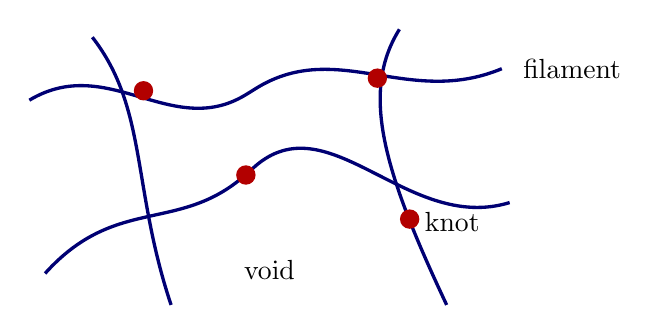
\begin{tikzpicture}[x=1cm,y=1cm]
  \draw[rounded corners=2pt,very thick,blue!45!black]
    (0.2,2.7) .. controls (1.2,3.3) and (2.0,2.2) .. (3.0,2.8)
    .. controls (4.1,3.5) and (5.0,2.6) .. (6.2,3.1);
  \draw[rounded corners=2pt,very thick,blue!45!black]
    (0.4,0.5) .. controls (1.3,1.5) and (2.1,1.0) .. (3.0,1.8)
    .. controls (4.0,2.7) and (5.0,1.0) .. (6.3,1.4);
  \draw[rounded corners=2pt,very thick,blue!45!black]
    (1.0,3.5) .. controls (1.7,2.6) and (1.5,1.6) .. (2.0,0.1);
  \draw[rounded corners=2pt,very thick,blue!45!black]
    (4.9,3.6) .. controls (4.4,2.8) and (4.7,1.8) .. (5.5,0.1);
  \fill[red!70!black] (1.65,2.82) circle (3.5pt);
  \fill[red!70!black] (4.62,2.98) circle (3.5pt);
  \fill[red!70!black] (2.95,1.75) circle (3.5pt);
  \fill[red!70!black] (5.03,1.19) circle (3.5pt);
  \node[align=center] at (3.25,0.55) {void};
  \node[right] at (6.35,3.1) {filament};
  \node[right] at (5.1,1.15) {knot};
\end{tikzpicture}
\caption{焦散網絡的清晰二維類比：線狀聚集圍出空洞，並在較明亮的節點處交會。在三維空間中，主要的摺疊形成片狀結構；片狀結構交會後形成絲狀結構和節點。}
\label{fig:c09-caustic-network}
\end{figure}

無外力的模型不能取代宇宙學微擾理論。引力對密度對比的增長、暈的形成、星系形成及非線性結構都至關重要。這個簡化模型單獨呈現一項穩健的幾何事實：略有變化的初始流場會自然摺疊並形成聚集。即使加入微小的初始密度變化，核心的雅可比論證也不會改變。

因此，我們只是把謎團往前推了一步，並沒有消除它。引入暴脹，是為了將一個區域拉伸到極其平坦、均勻。焦散計算假定初始流場具有微小的速度變化。這個非均勻的種子從何而來？下一講將探討暴脹期間場的量子漲落，並追問它們如何成為後來宇宙網的初始條件。

\section{這項論證確立了什麼}

均勻標量場的行為，就像一個在勢能\(V(\phi)\)中移動的座標。在固定盒子中，它遵循\(\ddot\phi=-V'(\phi)\)。在膨脹的共動盒子中，物理體積\(a^3\)會進入作用量，並導出
\[
\ddot\phi+3H\dot\phi=-V'(\phi).
\]
哈伯摩擦可以使場在高而平緩的勢能上維持緩慢的終端運動。此時場的動能變得微不足道，勢能使\(H\)近乎定值，而\(a(t)\)則近似呈指數增長。

膨脹稀釋了不需要的磁單極子，使幾何平滑，並驅使曲率趨近於零。然而，暴脹必須結束。場離開平臺、開始振盪，並將能量轉移給再加熱所產生的高溫粒子。仍有幾個問題尚未解答：勢能的形式、暴脹子的身分及其初始狀態、暴脹子與再加熱相關的耦合，以及今日觀測到的微小真空能。

暴脹的成功帶來最後一個問題：如果宇宙被完美地平滑化，就不會有星系。焦散映射
\[
y=x+v(x)t,
\qquad
\frac{dn}{dy}=\frac{1}{1+v'(x)t}
\]
顯示初始流場中的微小變化如何形成尖銳的片狀結構、絲狀結構和節點。但它並未解釋這些變化從何而來。接下來要探討的，正是它們的量子起源。
